% Created 2025-06-06 Fri 15:25
% Intended LaTeX compiler: pdflatex
\documentclass[aspectratio=169]{beamer}
\usepackage[utf8]{inputenc}
\usepackage[T1]{fontenc}
\usepackage{graphicx}
\usepackage{longtable}
\usepackage{wrapfig}
\usepackage{rotating}
\usepackage[normalem]{ulem}
\usepackage{amsmath}
\usepackage{amssymb}
\usepackage{capt-of}
\usepackage{hyperref}
\usepackage[style=apa, backend=biber]{biblatex}
\DeclareLanguageMapping{american}{american-apa}
\addbibresource{./refs/refs.bib}
\AtEveryBibitem{\clearfield{note}}
\usepackage{endnotes}
\let\footnote=\endnote
\usepackage{./jtc}
\usetheme{default}
\author{Evan Misshula}
\date{\today}
\title{Introduction to Machine Learning Workflow and Model Types}
\hypersetup{
 pdfauthor={Evan Misshula},
 pdftitle={Introduction to Machine Learning Workflow and Model Types},
 pdfkeywords={},
 pdfsubject={},
 pdfcreator={Emacs 29.3 (Org mode 9.6.15)}, 
 pdflang={English}}
\begin{document}

\maketitle

\section{Ingestion \& Preprocessing}
\label{sec:org2228b29}
\begin{frame}[label={sec:org2d9ebec}]{End to end process}
An \alert{ML workflow} is a sequence of steps to build and deploy a model that
solves a problem using data.
\end{frame}

\begin{frame}[label={sec:org7ad0784}]{The pipeline}
\begin{center}
\begin{tabular}{llll}
Ingestion \& Preprocessing & Analysis & Modeling & Deployment\\[0pt]
\hline
Definition & EDA & Selection & Tuning\\[0pt]
Data Collection & Feature Engineering & Training & Deployment\\[0pt]
Cleaning &  & Evaluation & Monitoring\\[0pt]
\end{tabular}
\end{center}

\begin{center}
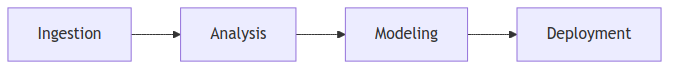
\includegraphics[width=.9\linewidth]{workflow.png}
\end{center}
\end{frame}

\begin{frame}[label={sec:org17d77d1}]{ML Workflow Graph}
\begin{center}
\begin{center}
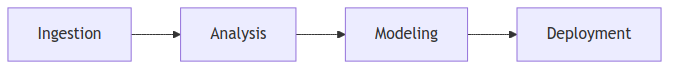
\includegraphics[width=.9\linewidth]{workflow.png}
\end{center}
\end{center}
\end{frame}
\section{Problem Definition}
\label{sec:org066f0ec}
\begin{frame}[label={sec:orgceab127}]{Define the problem}
\begin{itemize}
\item What are you trying to do?
\item Who is the end user of the prediction?
\item What decisions will be based on this output?

\item Predict tomorrow's temperature?
\item Predict a stock price?
\item Is this email spam?
\end{itemize}
\end{frame}
\begin{frame}[label={sec:org5401cb6}]{Classify or predict?}
\alert{Reminder} : the dependent variable is what you are trying to
predict

The other names are: response, "response variable", "regressand",
"criterion", "predicted variable", "measured variable", "explained
variable", "experimental variable", "responding variable", "outcome
variable", "output variable", "target" or "label".
\end{frame}

\begin{frame}[label={sec:orgfbb06b6}]{Classification vs Regression}
\alert{classification} aims to categorize data into distinct groups or
classes, while \alert{regression} involves estimating a continuous value, like
a number or a date.
\end{frame}

\begin{frame}[label={sec:org6153aa9}]{Classification vs Prediction Quiz}
\begin{itemize}
\item Housing prices?
\item If an individual is unhoused?
\item Is the email spam?
\item Will I get a job?
\item Income distribution of programmers?
\item Which party will win the Presential Election?
\end{itemize}
\end{frame}
\section{Collection}
\label{sec:org5af6bba}
\begin{frame}[label={sec:org0fac196}]{Data Collection}
\begin{itemize}
\item What do I have and how is it organized?
\begin{itemize}
\item What kind of file is it?
\begin{itemize}
\item CSV, JSON, Pickle, Excel Spreadsheet
\end{itemize}
\item Does my data exist in a database?
\begin{itemize}
\item Do I need SQL to retrieve it?
\end{itemize}
\item Is the data available through an API?
\begin{itemize}
\item In general better (more accurate, more frequent) data can be
expensive?
\item Do we think we will learn enough to justify the costs? Is the
project a demo or is there real money riding on the answer?
\end{itemize}
\end{itemize}
\end{itemize}
\end{frame}

\begin{frame}[label={sec:orgdfb935d}]{Data Collection tools}
Elementary libraries
\begin{itemize}
\item \alert{pandas} csv, json and some Relational Database
\item \alert{requests} good for well defined APIs
\item \alert{openpyxl} great way to import data from existing Excel Spreadsheets
\item \alert{SQL} if your data is in a relational database
\item \alert{BeautifulSoup} or \alert{Selenium} for web scraping (if needed)
\item \alert{duckdb} or \alert{sqlite} for lightweight DB queries
\end{itemize}
\end{frame}


\begin{frame}[label={sec:orgc519b59}]{Big Data Data Collection Tools}
Big Data \& Distributed Libraries
\begin{itemize}
\item \alert{PySpark} for distributed reading of CSV, JSON, Parquet, Avro, ORC files
\item \alert{Dask} scales pandas-like operations to multi-core or cluster setups
\item \alert{Apache Kafka} for real-time data ingestion from event streams
\item \alert{HDFS / S3 APIs} for direct access to distributed file systems
\item \alert{Delta Lake} / \alert{Iceberg} transactional layers on big data storage lakes
\item \alert{SQL Engines}: \alert{Hive}, \alert{Presto}, \alert{Trino}, \alert{Spark SQL} for querying
large-scale data
\end{itemize}
\end{frame}
\section{Data Cleaning}
\label{sec:org274e2a9}
\begin{frame}[label={sec:orgcd67cd6}]{Clean your data}
\alert{Data is always messier than you are told!}

\begin{itemize}
\item Be aware of missing values, outliers and duplicates
\item Verify your data types
\end{itemize}
\end{frame}

\begin{frame}[label={sec:orgcc00be1}]{Data Anomaly Definitions}
\begin{itemize}
\item \alert{Missing Values}: Observations where data is not recorded or
unavailable. Common causes include data entry errors, system
glitches, or sensor failures.

\item \alert{Outliers}: Data points that differ significantly from other
observations in the dataset. They may indicate variability in
measurement, experimental errors, or novel events.

\item \alert{Duplicates}: Records that appear more than once in a dataset but
represent the same real-world entity. These can bias results and
arise from repeated logging or failed deduplication.
\end{itemize}
\end{frame}
\begin{frame}[label={sec:org02c7bd7}]{Data Cleaning subtasks}
\begin{itemize}
\item Convert types (e.g., dates, categorical)

\item Don't normalize or scale numeric features (wait until modeling)

\item Detect inconsistent labels or typos in categorical data
\end{itemize}
\end{frame}


\begin{frame}[label={sec:org335fcb9}]{Never clean data by hand}
\begin{itemize}
\item Never clean your data by hand.  Always use scripts so that your
results can be reproduced.

\item Documentation is a way to be kind to your future self. The truth
is you will never remember why you did what did. Write it down!
\end{itemize}
\end{frame}

\section{Isolation Trees}
\label{sec:orga939dc3}
\begin{frame}[label={sec:org65c4d2e}]{Explanation of Isolation Forest}
\begin{itemize}
\item The isolation forest was introduced by Liu, Ting and Zhou in 2008.
\end{itemize}
\pause
\begin{itemize}
\item Now it's time for some math
\end{itemize}
\end{frame}

\begin{frame}[label={sec:org95aed9b}]{Isolation Forest: Mathematical Intuition}
\begin{block}{Problem Setting}
Given a dataset \(D = \{x_1, x_2, \ldots, x_n\} \subset \mathbb{R}^d\), the goal is to assign an \alert{anomaly score} \(s(x) \in [0, 1]\)
to each point \(x \in D\) based on how easily it can be
\alert{isolated}.
\end{block}
\end{frame}

\begin{frame}[label={sec:orgdae2e5d}]{Core Ideas}
\begin{itemize}
\item Anomalies are rare and different — they are easier to isolate.
\item Instead of profiling normal points, we attempt to isolate each point
using random partitions.
\item The \alert{fewer splits} needed to isolate a point, the more likely it is
to be an anomaly.
\end{itemize}
\end{frame}

\begin{frame}[label={sec:org147e460}]{Isolation Forest: Tree Construction}
\end{frame}

\begin{frame}[label={sec:orgfc58d2e}]{Isolation Tree Definition}
An \alert{isolation tree} is a binary tree where each node splits data based
on a randomly chosen feature and a randomly chosen split point within
that feature's range.
\end{frame}

\begin{frame}[label={sec:orgafa7f53}]{Sampling and Splitting}
\begin{enumerate}
\item Select a random subsample \(D_t \subset D\), of fixed size \(\psi\) (typically \(\psi = 256\)).

\item Recursively partition:
\begin{itemize}
\item Randomly select a feature index \(j \in \{1, \ldots, d\}\).
\item Choose a split point \(p \sim \text{Uniform}(\min x_j, \max x_j)\) for that feature.
\item Split the data: 
\[
     D_L = \{x \in D_t : x_j < p\}, \quad D_R = \{x \in D_t : x_j \geq p\}
     \]
\item Recurse on \(D_L\) and \(D_R\) until:
\begin{itemize}
\item Node contains a single instance, or
\item Tree reaches max depth \(\lceil \log_2 \psi \rceil\)
\end{itemize}
\end{itemize}
\end{enumerate}
\end{frame}

\begin{frame}[label={sec:orgc84093c}]{Isolation Forest: Scoring Mechanism}
\begin{block}{Path Length}
\begin{itemize}
\item For a point \(x\), the \alert{path length} \(h_t(x)\) is the number
of edges from the root of the tree to the leaf where \(x\) ends
up.
\end{itemize}
\end{block}

\begin{block}{Expected Path Length}
\begin{itemize}
\item The average path length over all trees:
\[
  E[h(x)] = \frac{1}{T} \sum_{t=1}^T h_t(x)
  \]
\end{itemize}
\end{block}

\begin{block}{Anomaly Score}
\begin{itemize}
\item The anomaly score is defined as:
\[
  s(x) = 2^{ - \frac{E[h(x)]}{c(\psi)} }
  \]
where:
\[
  c(\psi) = 2 H(\psi - 1) - \frac{2(\psi - 1)}{\psi}
  \]
and \(H(n) \approx \ln(n) + \gamma\) is the
\(n\)-th harmonic number,
with \(\gamma \approx 0.577\) (Euler–Mascheroni constant).
\end{itemize}
\end{block}
\end{frame}

\begin{frame}[label={sec:org54829f2}]{Interpretation}
\begin{block}{Interpreting the Score}
\begin{itemize}
\item \(s(x) \approx 1\): \(x\) is likely an \alert{outlier} (isolated in
fewer steps).
\item \(s(x) \approx 0\): \(x\) is likely \alert{normal} (harder to isolate).
\item Use a threshold (e.g., \(s(x) > 0.7\)) to flag anomalies.
\end{itemize}
\end{block}
\end{frame}


\begin{frame}[label={sec:org73c7a5d}]{Summary and Use}
\begin{itemize}
\item Unsupervised: Needs no labeled data
\item Fast, interpretable
\item Well-suited for high-dimensional data
\item Implementation: `sklearn.ensemble.IsolationForest`
\end{itemize}
\end{frame}
\end{document}
